\section{Confronto ore preventivate e ore effettive per ruolo}
\begin{frame}
	\frametitle{Confronto ore preventivate e ore effettive per ruolo}	
\begin{center}
	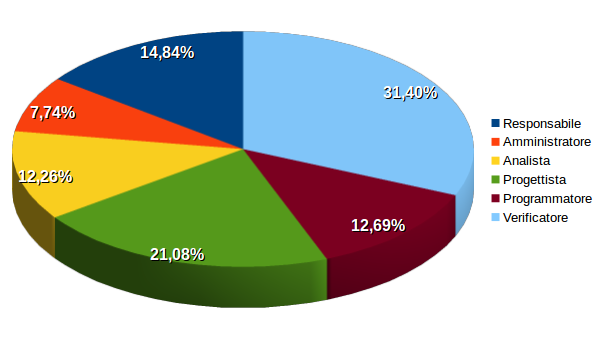
\includegraphics[scale=0.30]{img/orePREVENTIVATEperruolo.png}
	\qquad\qquad
	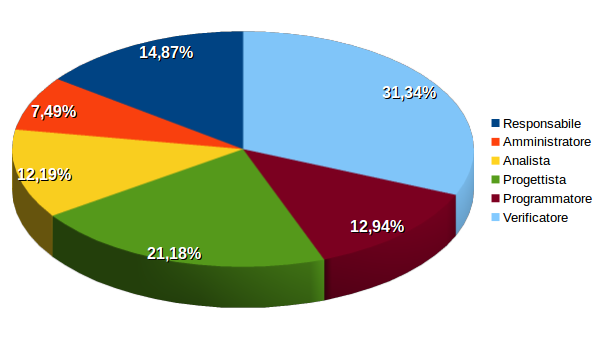
\includegraphics[scale=0.30]{img/oreEFFETTIVEperruolo.png}
\end{center}
	
	
\end{frame}

\section{Confronto costo preventivato e costo effettivo per ruolo}
\begin{frame}
	\frametitle{Confronto costo preventivato e costo effettivo per ruolo}	
	\begin{center}
		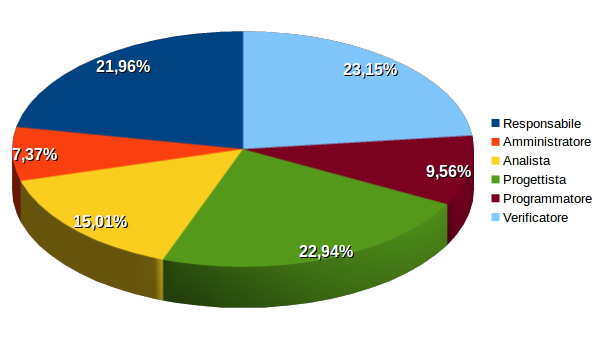
\includegraphics[scale=0.30]{img/costoEFFETTIVOperruolo.png}
		\qquad\qquad
		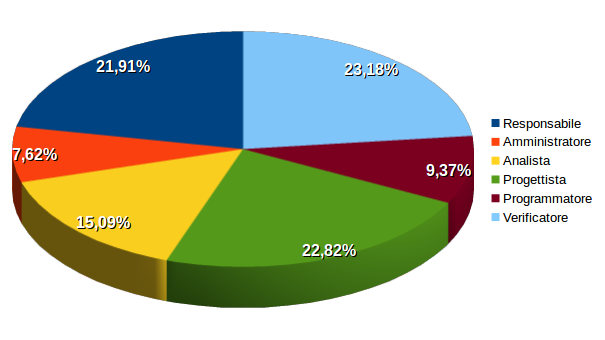
\includegraphics[scale=0.30]{img/costoPREVENTIVATOperruolo.png}
	\end{center}
	
	
\end{frame}


\section{Impegno individuale}
\begin{frame}
	\frametitle{Impegno individuale}	
	\begin{center}
		\centering
		\begin{tabular}{|c|c|c|}
			\hline
			\textbf{Nominativo} & \textbf{Ore preventivate} & \textbf{Ore effettive} \\
			\hline Emanuele Crespan	  & 107  & 107 \\
			\hline Tomas Mali  & 107  & 107  \\
			\hline Silvio Meneguzzo  & 106  & 106  \\
			\hline Nicolò Rigato  & 106  & 108  \\
			\hline Riccardo Saggese   & 107  & 108  \\
			\hline Federica Schifano  & 106  & 108  \\
			\hline
		
			\end{tabular}
		
	\end{center}
	
\end{frame}

\section{Consuntivo}
\begin{frame}
	\frametitle{Consuntivo}

\begin{center}
	\centering
	\begin{tabular}{|c|c|c|}
		\hline
		\textbf{Periodo} & \textbf{Preventivo} & \textbf{Consuntivo} \\
		\hline	\emph{Analisi dei requisiti}  &4425  &4425 \\
		\hline  \emph{Analisi in dettaglio}  &2180  &2165  \\
		\hline  \emph{Progettazione architetturale}  &2997  &2998  \\
		\hline  \emph{Progettazione in dettaglio}  &2830  &2884  \\
		\hline  \emph{Codifica}  &3665  &3680  \\
		\hline  \emph{Validazione}  &2795  &2834  \\
		\hline
		\textbf{Totale} &18892  & 18986  \\
		\hline
		\textbf{Rendicontato} &12287  & \textbf{12381} \\
		\hline
	\end{tabular}
	
\end{center}

\end{frame}